\chapter{Analysis}
	\section{Introduction}
		\subsection{Background}
I am creating this system for Sunny Future Solar, a trading name for Sunny
Future Ltd., a Company based in Aldershot, Hampshire, United Kingdom.  As
its name suggests, the Company installs solar panels, more specifically
solar photovoltaic panels, but it is a very small Company, having only two
full time employees who are also its directors: Philip and Angi Long.  The Company is accredited by the regulation body for all renewable technologies, the Microgeneration Certification Scheme (MCS).
		\subsection{Problem definition}
Sunny Future Solar must comply with the stringent documentation regulations laid out by the MCS.  This involves producing many documents (invoices, quotes, delivery logs, incident logs, survey forms, etc.) and keeping them all up to date.  Always having the correct versions of any one document, or indeed the same numbering system depending on who uses the computer, can be problematic as they do not follow the same personal guidelines, and one user is potentially more proficient (or patient!) than the other.  The current system does not have the ability to search documents or store central copies and have customer details stored.  The current system requires duplication of quotation and invoice data---Philip handwrites them and Angi types them up, and delivery\slash error log forms are filled in by hand.
		\subsection{The users}
Sunny Future Ltd.'s directors and employees will make use of the system.  One director, Philip Long, is the main worker in the business.  He has limited IT knowledge.  The second director, Angi Long, the secretary, has good knowledge of Microsoft Office, and adapts well.
	\section{Investigation of user needs and acceptable limitations}
		\subsection{The current system analysis}
			\subsubsection{Interview (1), 13\slash 10\slash 2011, 14:00}
During the first interview, I asked Angi Long, one of Sunny Future Solar's directors, the following questions and received the following responses:

Q: What is the current system?  What does it do?  What data is input and output?  How do you update it?\\
A: The current system has been developed from the requirements of the MCS and the REAL Consumer Code and practical situations during the last 17 months of trading.  The system deals predominantly with the contact with the customer from enquiry to final invoice, but also purchase ordering and an element of stock control.

Data input into and output from the current system:

\begin{tabular}{ | c | }
	\hline
\textbf{INPUT}\\
\hline
Customer details:\\
\hline
Name\\
Address\\
Postcode\\
Telephone Number\\
Email Address\\
Installation Address (if different)\\
MPAN No.\\
\hline
\end{tabular}
\begin{tabular}{ | c | }
\hline
\textbf{INPUT (again)}\\
\hline
Designed PV System Components:\\
\hline
kWp\\
Modules\\
Mounting\\
Inverter\\
\hline
Quotation No.\\
Net price\\
VAT\\ 
Total price\\
Required deposit on acceptance\\
Sap Calculation\\
FiT Calculations\\
Expected total benefit per year\\
Agreed Installation Date\\
Supplier Details\\
Purchase Order No.\\
Required Delivery Date\\
Goods-In\\
Component Serial Numbers\\
Invoice No.\\
Net price calculations\\
\hline
\end{tabular}
\begin{tabular}{ | c | }
	\hline
\textbf{OUTPUTS}\\
\hline
Initial Enquiry/Survey Form (Internal)\\
Covering Letter\\
Quotation\\
Quotation Log (Internal)\\
Benefit Sheet\\
Acknowledgement of Order\\
Receipt for deposit\\
Confirmation of Installation Date\\
Purchase Order\\
Purchase Log (Internal)\\
Goods-In sheet (Internal)\\
Final Invoice\\
Invoice Log (Internal)\\
Guarantee\\
\hline
\end{tabular}

Q: What are the problems with the current system?\\
A: Each element is currently added separately at each stage which takes time and is frustrating.

Q: What is your current IT infrastructure?  Would you be prepared to purchase additional software?\\
A: Sunny Future Solar work on Microsoft Windows on three computers, and use Microsoft Office 2007.  They would rather not spend money on software.  They also use Dropbox for shared filing, as their computers are not networked.

Q: Do you have a particular solution in mind?  Can you think of any possible constraints?\\
A: Fill in one database entry and for all the documentation, the relevant fields are completed by the database so that no repetition occurs with data entry.  However, the information must be able to be edited when necessary.
			\subsubsection{Observation}
\begin{itemize}
	\item{Sunny Future Solar received an enquiry.}
	\item{Angi arranged a time for Philip to visit the enquirer's house to conduct a survey of his roof and establish requirements.}
	\item{Angi filled in the customer's name, address, telephone number and email address on a printed paper copy of the survey form.}
	\item{Philip went to the house a few days later to conduct a survey.  After this, I went back to the office to further observe the process.}
	\item{The customer was keen, on the strength of Philip's comments when he did the survey, so Angi entered his details into a quotation document in Word, inputting them manually from the handwritten, printed survey form.}
	\item{Philip then sat down and handwrote the rest of the quotation, doing the necessary calculations (SAP, proposed price, deposit amount etc.) and specifying components according to the customer's wishes.  Angi then typed this quotation into the Microsoft Word document she had created beforehand.}
	\item{The quotation was then saved to the harddrive, implicitly backed up to Dropbox, and printed as hard copy twice: once for the customer, and once for Sunny Future Solar's customer paper folder, along with the hard copy of the survey form.}
	\item{The customer's copy of the quotation was sent to him that day.}
	\item{The customer accepted his quotation and paid his deposit a few days later, so I returned again.  Then, Angi was liasing with suppliers, organising delivery of components, and had fixed an installation date with the customer.}
	\item{The customer had his system installed two weeks later, and after that Angi typed an invoice, specifying the components actually used, the installation address (which in this case was the same as the billing address), and the final total price.  This was again saved and backed up, and printed twice, and sent to the customer.}
\end{itemize}
			\subsubsection{Investigation of documentation}
Sunny Future Solar provided me with various pieces of current system documentation.  Here are my findings:

Their current documentation is paper-based, so hard to manage as multiple people, for example the two directors, cannot have multiple copies of the same piece of paper with the same data on it, so inconsistencies between numbering of entries in forms arise, for example.  With regard to the MCS accreditation, Sunny Future Solar are required to keep copies of various reports, forms and strategies to comply with regulations, along with a document master list with all document numbers which is very intricate.  These documents require lots of data to be input into several documents, so it is not practical to do it by hand---they need a system which will take data from one form and put it where it is meant to go in another according to certain conditions.
			\subsubsection{Investigation of input forms, output forms and report formats from the existing system}
Sunny Future Solar provided me with various pieces of documentation: a quotation, an invoice, a quality plan, a potential benefits sheet, a cancellation form, a survey form, a job sheet, a purchase form, a purchased order log sheet, and the MCS master documentation list.

The potential benefits sheet is a sheet mostly made up of static text, just with the SAP calculation (which is different for every person, so at the moment requires manual entry) inserted.\\
The job sheet duplicates some of the information contained on the survey form.\\
The purchase form indicates the order number, the order date, the components sought, the shipping cost, and the total cost, and the delivery date.  This is filled in by Sunny Future Solar after every order for components is placed.\\
The purchase order log sheet is used to record when Sunny Future Solar receives the shipment.\\
		\subsection{Data Flow Diagram of the current system}
Here are the data flow diagrams (level 0 to level 1) that I devised based on the process documents for an installation plan that Sunny Future Solar provided.

\textsl{In these diagrams and `Data sources and destinations', Sunny Future Solar is referred to as `SFS'.}

Level 0:\\
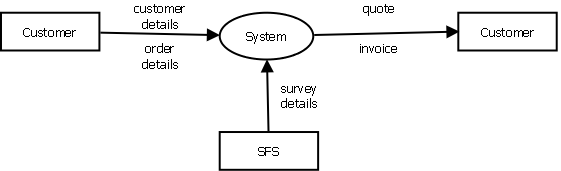
\includegraphics[scale=0.5]{dfd_old_zero_n}

Level 1:\\
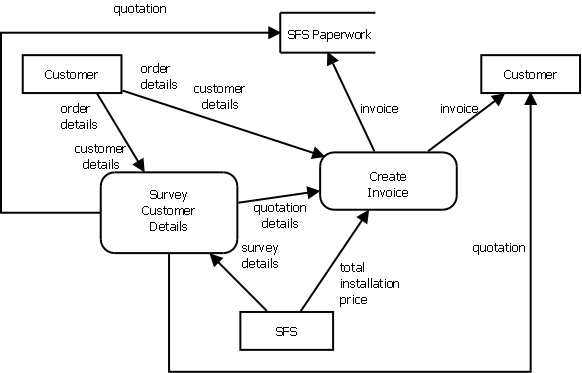
\includegraphics[scale=0.45]{dfd_old_one_n}
		\subsection{Data sources and destinations}

The first data source is the customer: he or she gives the order details and his or her personal details (address, name, email address\ldots) to SFS, which goes onto a survey form.  The survey form details are used by SFS to produce a quotation which gets printed and stored in the SFS paperwork customer folder, and also posted to the customer.  The quotation, as well as being an output, is also used as a data source for the invoice after the job is done: component details and customer details are taken from that quotation, adapted if necessary depending on what was really installed, and again stored in SFS's paper customer folder, and printed and sent to the customer for payment and their own records.  SFS is also a data source as they provide component details frmo their suppliers, and price and deposit details.
		\subsection{Entity relationship diagram and entity descriptions of the current system}

\textbf{Paper\slash brain-based.}

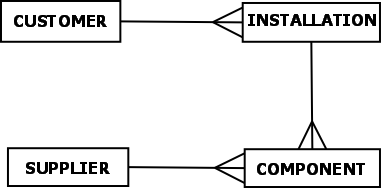
\includegraphics[scale=0.45]{erd_new}

Every customer can have many installations; Each installation can only be
installed on one customer's roof.\\
Every installation can have many components. Each component can only be
fitted onto one installation.\\
Every supplier can supply many components.  Each component can only be
supplied by one, specialist supplier (the best one).

		\subsection{Discussion of problems with the current system}
The current system is fragmented, open to data entry duplication and error, and not sufficiently efficient for a successful solar panel installation business.
		\subsection{The proposed new system analysis}
			\subsubsection{User needs}
Much of the data included on one paper form (a quotation, for instance, or an
order job sheet) is repeated---name, address, calculations and panel
details are examples.  This data needs to be stored in a centralised
database so that the data is not repeated
unnecessarily due to the fact that Sunny Future Solar operates from three
different computers: one desktop in their office, plus two laptops.  The
user needs not to waste too much time so that he or she can spend more time
finding customers, and the fewer minutes or hours he or she wastes entering data, the
fewer times he or she has to enter it, logically, so lessening the number
of potential data entry errors.  Reports have to be created: quotations, invoices, logs and survey forms.  These will require Microsoft Word compatibility and printing.
			\subsubsection{Interview (2), 24\slash 10\slash 11, 19:00}
Q: What should the new system actually do?\\
A: The new system requires the creation of a database to record the information above.  It should also hold write only `field' versions of the paperwork required, automatically completed by the database record ready for use.

Q: What reports are required---would you like it to work with Word?\\
A: Reporting is required: logs are completed (see above), along with invoices and quotations.  It would need to work with Microsoft Word (oepning, editing, etc.).

Q: How much data will the system hold per section?\\
A: A potential maximum of 500 records per year.
		\subsection{Data Flow Diagram of the proposed new system}
Here is the level 1 data flow diagram that I devised based on my research and investigation into what Sunny Future Solar's new system will be.

\textsl{In this diagram, Sunny Future Solar is referred to as `SFS'.}

Level 1:\\
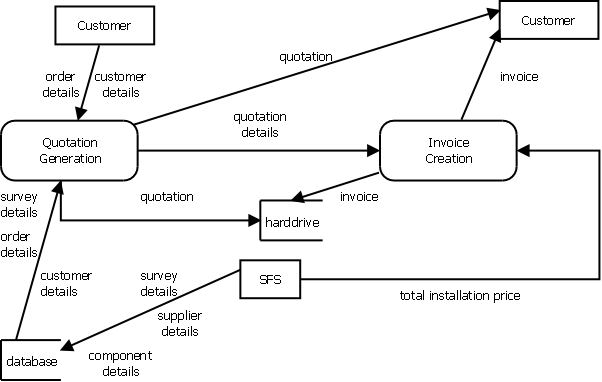
\includegraphics[scale=0.35]{dfd_new_one_n}
		\subsection{Data sources and destinations}
The first data source is the customer: he or she gives the order details and his or her personal details (address, name, email address\ldots) to SFS, which goes onto a survey form.  The survey form details are used by SFS to produce a quotation which gets printed and stored on the computer's harddrive, and also posted to the customer.  The quotation, as well as being an output, is also used as a data source for the invoice after the job is done: component details and customer details are taken from that quotation, or the database, adapted if necessary depending on what was really installed, and again stored in SFS's computer file system, and printed and sent to the customer for payment and their own records.  SFS is also a data source as they provide component details frmo their suppliers, and price and deposit details, though these are in the database via the program.
		\subsection{Entity relationship diagram and entity descriptions of the new system}
\textbf{Computer\slash database-based.}

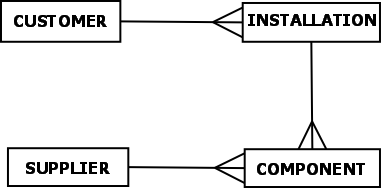
\includegraphics[scale=0.45]{erd_new}

Every customer can have many installations; Each installation can only be
installed on one customer's roof.\\
Every installation can have many components. Each component can only be
fitted onto one installation.\\
Every supplier can supply many components.  Each component can only be
supplied by one, specialist supplier (the best one).

\textit{Customer}(\underline{cust\_id}, cust\_title, cust\_name, cust\_billaddress, cust\_billpostcode, cust\_instaddress, cust\_instpostcode, cust\_hometelno, cust\_mobtelno, cust\_mpan, cust\_email)\\
\textit{Supplier}(\underline{supp\_id}, supp\_name, supp\_address, supp\_postcode, supp\_telno, supp\_contactname)\\
\textit{Component}(\underline{comp\_id}, comp\_name, comp\_type, comp\_serialno, comp\_panelwp, comp\_supplier*)\\
\textit{Installation}(\underline{inst\_id}, inst\_netprice, inst\_vat, inst\_totalprice, inst\_deposit, inst\_dateinstall, inst\_sapcalc, inst\_purchordernum, inst\_deliverydate, inst\_invoiceno, cust\_id*)

This database is in the first normal form (1NF) because every piece of data is atomic, i.e. there are no repeating groups.\\
The database is in the second normal form (2NF) because it is in the first normal form (1NF) and there are no partial key dependencies.\\
The database is in the third normal form (3NF) because it is in the second normal form (2NF) and contains no non-key dependencies.
		\subsection{Analysis data dictionary}
Customer:

\begin{center}
	\begin{longtable}{ | p{4cm} | p{4cm} | p{4cm} | p{4cm} | }
		\hline
		\textbf{Item Name} & \textbf{Data Type} & \textbf{Size
(chars)} & \textbf{Example}\\
		\endfirsthead
		\hline
		\textbf{Item Name (cont.)} & \textbf{Data Type (cont.)} &
\textbf{Size (chars) (cont.)} & \textbf{Example (cont.)}\\
		\endhead
		\hline
		Surname & String & 25 & Long\\
		\hline
		Forename & String & 22 & Isabell\\
		\hline
		Address & String & 100 & 12 Reputable Place\\
		\hline
		TelNum & String & 13 & 01234 567890\\
		\hline
		Email & String & 25 & example@example.com\\
		\hline
		InstallAddress & String & 100 & 54 SolarInstall Place\\
		\hline
		MPANNumber\footnotemark & Integer & 32 (bits) & 00012345678901\\
		\hline
	\end{longtable}
\end{center}
\footnotetext[1]{The MPAN number is the number that uniquely identifies every electricity supply point (individual domestic, for example) in the UK.}

Component:

\begin{center}
	\begin{longtable}{ | p{4cm} | p{4cm} | p{4cm} | p{4cm} | }
		\hline
		\textbf{Item Name} & \textbf{Data Type} & \textbf{Size
(chars.)} & \textbf{Example}\\
		\endfirsthead
		\hline
		\textbf{Item Name (cont.)} & \textbf{Data Type (cont.)} &
\textbf{Size (chars.) (cont.)} & \textbf{Example (cont.)}\\
		\endhead
		\hline
		PanelName (module) & String & 20 & Sanyo\\
		\hline
		PanelType (module) & Integer & 32 (bits) & 235\\
		\hline
		Watts & Integer & 32 (bits) & 3250\\
		\hline
		Mounting (frame) & String & 20 & Renusol \\
		\hline
		InverterName & String & 15 & SMA\\
		\hline
		InverterType & String & 20 & SB1700TL\\
		\hline
		SerialNumber & String & 10 & SEN1024854\\
		\hline
		BracketType & String & 10 & Bracket001\\
		\hline
	\end{longtable}
\end{center}

Supplier:

\begin{center}
	\begin{longtable}{ | p{4cm} | p{4cm} | p{4cm} | p{4cm} | }
		\hline
		\textbf{Item Name} & \textbf{Data Type} & \textbf{Size
(chars.)} & \textbf{Example}\\
		\endfirsthead
		\hline
		\textbf{Item Name (cont.)} & \textbf{Data Type (cont.)} &
\textbf{Size (chars.) (cont.)} & \textbf{Example (cont.)}\\
		\endhead
		\hline
		SupplierName & String & 25 & Alternergy\\
		\hline
		SupplierAddress & String & 100 & 25 Supplier Place\\
		\hline
		SupplierTelNo & String & 13 & 01234 567890\\
		\hline
		SupplierContactName & String & 25 & Alex Wright\\
		\hline
	\end{longtable}
\end{center}

Installation:

\begin{center}
	\begin{longtable}{ | p{4cm} | p{4cm} | p{4cm} | p{4cm} | }
		\hline
		\textbf{Item Name} & \textbf{Data Type} & \textbf{Size
(chars.)} & \textbf{Example}\\
		\endfirsthead
		\hline
		\textbf{Item Name (cont.)} & \textbf{Data Type (cont.)} &
\textbf{Size (chars.) (cont.)} & \textbf{Example (cont.)}\\
		\endhead
		\hline
		QuotationNumber & Integer & 32 (bits) & 001234\\
		\hline
		NetPrice (\pounds) & Integer & 32 (bits) & 10000\\
		\hline
		VAT (\%) & Integer & 32 (bits) & 5\\
		\hline
		TotalPrice (\pounds) & Integer & 32 (bits) & 15000\\
		\hline
		DepositAmount (\pounds) & Integer & 32 (bits) & 500\\
		\hline
		AgreedInstallDate & Date & 10 & 03/04/2012\\
		\hline
		SAPCalc\footnotemark & String & 20 & 0.8$\times$2.9$\times$1073$\times$0.8\\
		\hline
		PurchaseOrderNum & Integer & 32 (bits) & 12345678909876543210\\
		\hline
		DeliveryDate & Date & 10 & 02/03/2012\\
		\hline
		InvoiceNumber & Integer & 32 (bits) & 001234\\
		\hline
	\end{longtable}
\end{center}
\footnotetext[2]{The SAP calculation is the calculation devised by the government to ensure that solar installation companies do not over extol the Feed in Tariff benefits of solar PV.}
		\subsection{Data volumes}
		
Sunny Future Solar estimate a maximum of five hundred customers per year, so a maximum of five hundred customers will be inserted into the Customer table.  Sunny Future Solar alternate between suppliers, but have seven main suppliers at present, therefore a theoretical maximum of thirty suppliers in the supplier table.  As for components, many, many components exist, not all of them available at the same time; therefore, a realistic estimate for components (from the thirty suppliers) is six hundred, for the component table (600$/$30).
	\section{Constraints}
		\subsection{Hardware constraints}
Sunny Future Solar operate from three reasonably new computers: two laptops and a desktop in their office.  Therefore, the computer that this program will be running on will be up-to-date enough to handle it.
		\subsection{Software constraints}
All Sunny Future Solar's computers are equipped with versions of Microsoft Windows, either Vista or 7, and Microsoft Office 2007, so there will be no problem with software versions.
		\subsection{Time constraints}
The system has to be built in months, not years: precisely, I have until April 2012 to build the system.  Due to this, I may not have time to implement all the features that my user would like: this analysis has been an attempt at creating realistic targets. 
		\subsection{User's knowledge of information technology}
The users have reasonable knowledge of information technology: they use Microsoft Windows computers on a daily basis, and are proficient with Microsoft Word.
		\subsection{Who will be allowed to use various parts of the system}
Philip and Angi Long will be allowed to use the system, and future employees will be able to access certain parts of the system if authorised by Philip or Angi to do so.
	\section{Limitations}
		\subsection{Areas which will not be included in computerisation}
		\begin{itemize}
			\item{Implementation of a stock control system.}
		\end{itemize}
		\subsection{Areas considered for later development}
		\begin{itemize}
			\item{Implementation of a stock control system.}
			\item{Cross-platform compatibility.}
		\end{itemize}
	\section{Objectives}
		\subsection{General objectives}
		\begin{itemize}
			\item{Streamline the efficiency of the administration process within Sunny Future Solar.}
		\end{itemize}
		\subsection{Specific objectives}
		\begin{enumerate}
			\item{Have a main menu that allows the user to
select different options.}
			\item{Have a functioning relational database,
queriable with runtime SQL, made in Microsoft Access, with the required number of
tables.}
			\item{Enable the user to add customers.}
			\item{Enable the user to add suppliers.}
			\item{Enable the user to add components.}
			\item{Enable the user to remove customers.}
			\item{Enable the user to remove suppliers.}
			\item{Enable the user to remove components.}
			\item{Enable the user to list customers.}
			\item{Enable the user to list suppliers.}
			\item{Enable the user to list components.}
			\item{Enable the user to view and edit invoices, log forms,
and reports in Microsoft Word by clicking buttons in the program to open
the requested forms.}
			\item{Enable the user to view relationships between
suppliers and the components they stock.}
			\item{The program must input data into the invoices
and quotes to avoid the user having to duplicate data entry, and this data
must come from either user input or data from the database.}
			\item{The system should be menu-driven, with
consistent GUI form layout throughout, as far as possible.}
			\item{Enable printing directly from the program for
the user to print lists of customers etc.}
			\item{Enable searching of customers, suppliers and components, and sort the search results.}
		\end{enumerate}
	\section{Consideration of alternative solutions}
The proposed solution is to write the system in Visual Basic.NET with a
Visual Basic forms GUI
frontend, a Microsoft Access database, and Microsoft Office integration for
the reports.  An alternative solution would be to not build a bespoke system but use an already built system such as SAGE, but, for Sunny Future Solar who have minimal amounts of data to input and manipulate, such a big and complex system would take up unnecessary space and cost unnecessarily large amounts of money.  Another alternative solution would be to code the solution in a language other than VisualBasic.NET, enabling cross-platform compatibility, however Visual Basic is the language I am most familiar with, and no operating systems other than Windows run on any of Sunny Future Solar's office computers.
	\section{Justification of the chosen solution}
Building the system in VisualBasic.NET is best because a fully documented
system will be available and the developer of the system will be available
to fix the system if it goes wrong, which would not be possible if they
were to use an already built package developed by someone remote as
mentioned above.  Also, features will be able to more easily be added as
and when the user wants them, rather than having to go through a
potentially slow process of emails and phone calls to invisible people.  VisualBasic.NET is the language I feel most comfortable with, and Sunny Future Solar require easy integration with Microsoft Word which works well with VB.NET.
